%*********************************************************
% Änderung vom 09.11.11: Bisherige Definition entfernt und durch
% Definition von Prof. Schmidt ersetzt. (js75)
%*********************************************************
\subsection{Definition}
Eine \emph{Abbildung} $f$ besteht aus drei Teilen: einer Ausgangsmenge $A$
(genannt \emph{Definitionsbereich}), einer Zielmenge $B$ (genannt
\emph{Wertebereich}) und einer Abbildungsvorschrift $x \overset{f}{\mapsto}
f(x)$. Jedem Element $x$ aus $A$ kann \underline{genau ein} Element $y = f(x)
\eqcolon fx$ aus $B$ zugeordnet werden.

\subsubsection{Beispiel}
$A$ = Menge von Personen, $B$ = Menge von Jahreszahlen und $x \mapsto
fx$\\
Jeder Person $x$ aus $A$ wird ihr Geburtsjahr $y = fx$ aus $B$ zugeordnet.

\subsubsection{Notation}
Ist $f$ eine Abbildung mit Ausgangsmenge $A$ und Zielmenge $B$, so schreiben
wir $f \colon A \rightarrow B, x \mapsto fx$ anstelle von $f$.

Mit $\Def(f) \coloneq A$ und $\Wert(f) \coloneq B$ können wir auch
für $f$ die Notation $f \colon \Def(f) \rightarrow \Wert(f), x
\mapsto fx$ verwenden.

\paragraph{Anmerkungen}
\begin{enumerate}[(a)]
  \item Abbildung = map oder mapping
  \item Funktion = function (ist immer eine Abbildung, \underline{manchmal}
  synonym, manchmal spezieller)
\end{enumerate}

Von bijektiven Funktionen kann eine \emph{Umkehrfunktion} $f^{-1} :
{B}\rightarrow{A} $ gebildet werden. Deswegen bezeichnet bijektive
Funktionen auch als \emph{invertierbar}.

Diese ist nicht zu verwechseln mit dem \emph{Urbild}, was ähnlich geschrieben
wird.

\subsubsection*{Beispiel}
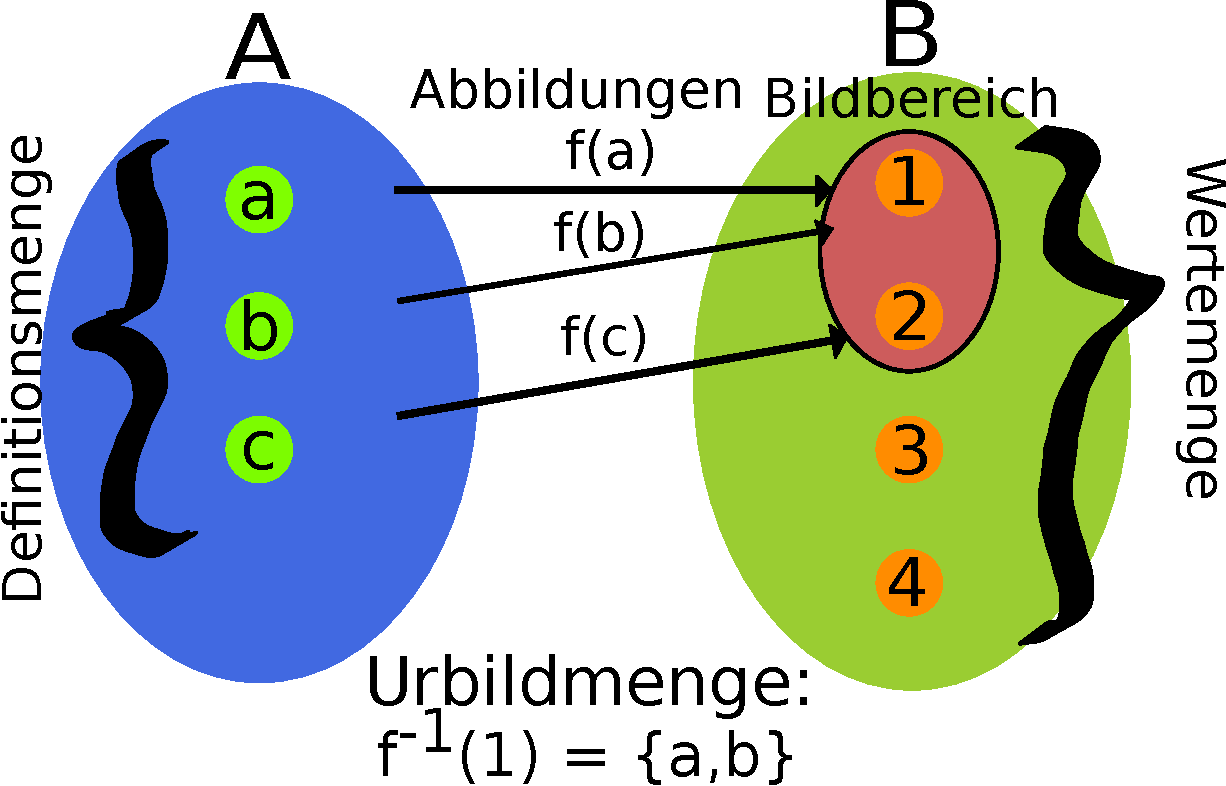
\includegraphics[scale=0.5]{abbildung.pdf}
%%% Local Variables:
%%% mode: latex
%%% TeX-master: "../script"
%%% End:

\paragraph{Hinweis:}
Der Begriff \emph{Wertemenge} kann als Synonym sowohl für die \emph{Zielmenge}
als auch für den \emph{Bildbereich} verwendet werden. In diesem Skript sind
\emph{Zielmenge} und {Wertemenge} identisch, der \emph{Bildbereich} ist somit
eine Teilmenge der \emph{Wertemenge} (siehe auch Abschnitt ~\ref{kap_typabb}).
